\section{Волновые уравнения}
\subsection{Однородное одномерное волновое уравнение в неограниченной среде с заданными начальными условиями}

Как оно выглядит? Да, вот так:
\[
	\dfs{u}{x} - \frac{1}{v^2} \dfs{u}{t} = 0
\]
В обычном случае $v = const$. Начальные условия:
\[
	\begin{aligned}
		& u(0, x) = f(x) \\
		& \dff{u}{t} \Big|_{(0, x)} = g(x)
	\end{aligned}
\]
Его очень легко решить, если воспользоваться заменой координат:
\[
	\begin{aligned}
	& \eta = x + v t \\
	& \xi = x - v t
	\end{aligned}	
\]
\[
	\begin{aligned}
		& \dff{u}{x} = \dff{u}{\eta} \dff{\eta}{x} + \dff{u}{\xi} \dff{\xi}{x} =
			\dff{u}{\eta} + \dff{u}{\xi} \\
		& \dfs{u}{x} = \dfs{u}{\eta} \dff{\eta}{x} + \dfss{u}{\xi}{\eta} \dff{\xi}{x} + \dfss{u}{\eta}{\xi} \dff{\eta}{x} +  \dfs{u}{\xi} \dff{\xi}{x} =
			\dfs{u}{\eta} +  \dfs{u}{\xi} + 2 \dfss{u}{\xi}{\eta} \\
		& \dff{u}{t} = \dff{u}{\eta} \dff{\eta}{t} + \dff{u}{\xi} \dff{\xi}{t} =
			v \left(\dff{u}{\eta} - \dff{u}{\xi}\right) \\
		& \dfs{u}{t} = v\dfs{u}{\eta} \dff{\eta}{t} + v\dfss{u}{\xi}{\eta} \dff{\xi}{t} - v\dfss{u}{\eta}{\xi} \dff{\eta}{t} -  v\dfs{u}{\xi} \dff{\xi}{t} =
		v^2\left(\dfs{u}{\eta} +  \dfs{u}{\xi} - 2 \dfss{u}{\xi}{\eta} \right)\\ 
	\end{aligned}
\]
\[
	\dfs{u}{x} - \frac{1}{v^2} \dfs{u}{t} = 4 \dfss{u}{\xi}{\eta} = 0
\]
\[
	\dff{u}{\eta} = U_1(\eta)
\]
\[
	u = U(\eta) + V(\xi)
\]
\[
	\begin{aligned}
	& u(0, x) = U(x) + V(x) = f(x) \\
	& \dff{u}{t} \Big|_{(0, x)} = v \left(U'(x) - V'(x)\right) = g(x)
	\end{aligned}
	\Rightarrow
	\begin{aligned}
	& U(x) + V(x) = f(x) \\
	& U(x) - V(x) = \frac{1}{v} \int g(x) dx = \frac{G(x)}{v}
	\end{aligned}
\]
\[
	u = \frac{f(x + v t) + f(x - v t)}{2} + \frac{G(x + v t) - G(x - v t)}{2 v} = \frac{f(x + v t) + f(x - v t)}{2} + \frac{1}{2 v} \int\limits_{x - v t}^{x + v t} g(x) dx
\]

\subsection{Метод преобразования Фурье для неоднородного одномерного волнового уравнения в бесконечной среде с нулевыми начальными условиями}

\[
\dfs{u}{x} - \frac{1}{v^2} \dfs{u}{t} = s(x, t)
\]
$v = const$. Начальные условия:
\[
	\begin{aligned}
	& u(0, x) = 0 \\
	& \dff{u}{t} \Big|_{(0, x)} = 0
	\end{aligned}
\]
Только координата $x$ меняется от $-\infty$ до $\infty$, поэтому преобразование Фурье будет иметь вид:
\[
	\begin{aligned}
	& u(x, t) = \int\limits_{-\infty}^{\infty} U(k, t) e^{-ikx} dk \qquad\Leftrightarrow \qquad  U(k, t) = \frac{1}{2\pi}\int\limits_{-\infty}^{\infty} u(x, t) e^{ikx} dx\\
	& s(x, t) = \int\limits_{-\infty}^{\infty} S(k, t) e^{-ikx} dk
	\qquad\Leftrightarrow \qquad
	S(k, t) = \frac{1}{2\pi}\int\limits_{-\infty}^{\infty} s(x, t) e^{ikx} dx
	\end{aligned}
\]
Выполняем преобразование Фурье исходного уравнения:
\[
	\frac{1}{2\pi} \int\limits_{-\infty}^{\infty}\dfs{u}{x} e^{ikx} dx = 
	\frac{1}{2\pi} \dff{u}{x} e^{ikx} \Big|_{-\infty}^{\infty} - 
	\frac{ik}{2\pi} \int\limits_{-\infty}^{\infty}\dff{u}{x} e^{ikx} dx =
	\frac{1}{2\pi} \left(\dff{u}{x} - ik u \right) e^{ikx} \Big|_{-\infty}^{\infty}
	- k^2 U
\]
При условии, что:
\[
	 \lim\limits_{x \to \pm \infty }\left(\dff{u}{x} - ik u \right) = 0
\]
получаем преобразованное уравнение:
\[
	- k^2 U - \frac{1}{v^2} \Dfs{U}{t} = S(k, t)
\]
И начальные условия:
\[
	\begin{aligned}
	& U(k, 0) = 0 \\
	& \Dff{U}{t} \Big|_{(k, 0)} = 0
	\end{aligned}
\]
Решение этого уравнения:
\[
	U(k, t) = - \frac{v}{k} \int\limits_{0}^{t} \sin(vk (t - t')) S(k, t') dt'
\]
\[
	\begin{gathered}
	u(x, t) = -\int\limits_{0}^{t} \! \int\limits_{-\infty}^{\infty} \frac{v}{k} \sin(vk (t - t')) S(k, t') e^{-ikx}  dk\, dt' =
	-\int\limits_{0}^{t} \! \int\limits_{-\infty}^{\infty} \! \int\limits_{-\infty}^{\infty} \frac{v}{2k\pi} \sin(vk (t - t')) s(x', t') e^{-ik(x - x')}  dk\, dt'\, dx' = \\ =
	-\frac{v}{4} \int\limits_{0}^{t}  \! \int\limits_{-\infty}^{\infty} [ \sign (x - x' + v(t - t')) - \sign (x - x' - v (t - t')) ] s(x', t') dt' dx' = \\ =
	-\frac{v}{4} \int\limits_{0}^{t} \! \int\limits_{-\infty}^{\infty} [ \sign (\xi + v \tau) - \sign (\xi - v\tau) ] s(x - \xi, t - \tau) d\tau d\xi 
	\end{gathered}
\]
\[
	\begin{aligned}
	\sign (x + a) - \sign (x - a) = 
	\begin{cases}
	\left\{
	\begin{aligned}
	& 0, & x > a, \\
	& 1, & x = a, \\
	& 2, & -a < x < a, \\
	& 1, & x = - a, \\
	& 0, & x < - a.
	\end{aligned}
	\right\},
	& a > 0, \\
	0,
	& a = 0, \\
	\left\{
	\begin{aligned}
	& 0, & x > - a, \\
	& -1, & x = - a, \\
	& -2, & a < x < -a, \\
	& -1, & x = a, \\
	& 0, & x < a.
	\end{aligned}
	\right\},
	& a < 0. \\
	\end{cases}
	=
	\begin{cases}
	0, & |x|>|a|, \\ 
	\sign(a), & |x|=|a|, \\ 
	2 \sign(a), & |x| < |a|.
	\end{cases}
	=
	2 \eta(|a| - |x|) \sign(a)
	\end{aligned}
\]
\[
	 \sign (\xi + v \tau) - \sign (\xi - v\tau) = 2 \eta(v|\tau| - |\xi|) \sign(v\tau)
\]
\[
	\begin{aligned}
	u(x, t) =
	-\frac{v}{2} \int\limits_{0}^{t} \! \int\limits_{-\infty}^{\infty} \eta(v|\tau| - |\xi|) \sign(v\tau) s(x - \xi, t - \tau) d\tau\, d\xi = \\ =
	[\text{если, $s(x - \xi, t - \tau)$ не имеет $\delta$-образных разывов}] = \\ =
	-\frac{v}{2} \int\limits_{0}^{t} \! \int\limits_{-v\tau}^{v\tau} s(x - \xi, t - \tau) d\tau\, d\xi
	\end{aligned}
\]
%Проверим, что найденное решение удовлетворяет уравнению:
%\[
%	\begin{gathered}
%	\dfs{u}{x} - \frac{1}{v^2} \dfs{u}{t} =
%	-\frac{v}{2} \int\limits_{0}^{t} \! \int\limits_{-\infty}^{\infty} \eta(\tau - |\xi|/v)
%	\left(\dfs{}{x} - \frac{1}{v^2} \dfs{}{t}\right) s(x - \xi, t - \tau) d\tau\, d\xi = \\ =
%	-\frac{v}{2} \int\limits_{0}^{t} \! \int\limits_{-\infty}^{\infty} \eta(\tau - |\xi|/v)
%	\left(\dfs{}{\xi} - \frac{1}{v^2} \dfs{}{\tau}\right) s(x - \xi, t - \tau) d\tau\, d\xi
%	\end{gathered}
%\]

\subsection{Примеры}

\textbf{1. Пусть:}
\[
s(x, t) = \delta(x - x_0) \delta (t - t_0) 
\]
что соответствует импульсу, мгновенно переданному отдельной точке струны.
\[
\begin{gathered}
u(x, t) =
-\frac{v}{4} \int\limits_{0}^{t} \! \int\limits_{-\infty}^{\infty} [ \sign (\xi + v \tau) - \sign (\xi - v\tau) ] s(x - \xi, t - \tau) d\tau d\xi =
\\ =
-\frac{v}{4} \int\limits_{0}^{t} \! \int\limits_{-\infty}^{\infty} [ \sign (\xi + v \tau) - \sign (\xi - v\tau) ] \delta(x - x_0 - \xi) \delta (t - t_0 - \tau)  d\tau d\xi =
\\ =
-\frac{v}{4} \int\limits_{0}^{t}  [ \sign (x - x_0 + v \tau) - \sign (x - x_0 - v\tau) ] \delta (t - t_0 - \tau)  d\tau = 
\\ =
-\frac{v}{4} [ \sign (x - x_0 + v (t - t_0)) - \sign (x - x_0 - v(t - t_0)) ] \eta(t - t_0)
\end{gathered}
\]
Проверяем:
\[
\dfs{u}{x} = - \frac{v}{2} [\delta' (x - x_0 + v (t - t_0)) - \delta' (x - x_0 - v(t - t_0))]\eta(t - t_0)
\]
\[
\begin{gathered}
\dfs{u}{t} = -\frac{v}{4} \left\{
2 v^2 [\delta' (x - x_0 + v (t - t_0)) - \delta' (x - x_0 - v(t - t_0)) ] \eta(t - t_0) +
\right.\\ + \left.
4 v [\delta (x - x_0 + v (t - t_0)) + \delta (x - x_0 - v(t - t_0))]\delta(t - t_0) +
\right.\\ + \left.
[ \sign (x - x_0 + v (t - t_0)) - \sign (x - x_0 - v(t - t_0)) ] \delta'(t - t_0)
\right\}
\end{gathered}
\]
Воспользуемся тождествами:
\[
f(x)\delta(x - x_0) + [F(x) - F(x_0)] \delta'(x - x_0) = 0, \qquad F(x) = \int f(x) dx
\]
\[
f(x) \delta(x -x_0) = f(x_0) \delta(x - x_0)
\]
Кое-что подсократилось:
\[
\begin{gathered}
\dfs{u}{t} = -\frac{v}{4} \left\{
2 v^2 [\delta' (x - x_0 + v (t - t_0)) - \delta' (x - x_0 - v(t - t_0)) ] \eta(t - t_0) +
\right.\\ + \left.
4 v \delta (x - x_0) \delta(t - t_0)
\right\}
\end{gathered}
\]
\[
\Rightarrow
\dfs{u}{x} - \frac{1}{v^2} \dfs{u}{t} = \delta (x - x_0) \delta(t - t_0)
\]
На рисунке показан профиль струны в различные моменты времени:
\begin{center}
	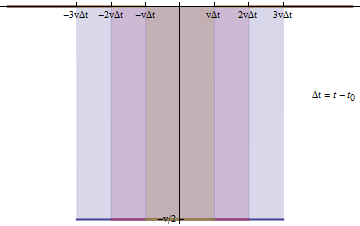
\includegraphics[width=0.5\textwidth]{images/png/for_delta_force.png}
\end{center}

\textbf{Одно тождество}

Рассмотрим функцию вида:
\[
	u(x, t) = \eta(t - t_0) \eta(\xi) f(\xi), \text{ если } \xi = t - t_0 - |x - x_0|/v 
\]
\[
	\begin{gathered}
	u''_{tt} = 
	\delta'(t - t_0) \eta(\xi) f(\xi) + 
	2 \delta(t - t_0) (\delta(\xi) f(\xi) + \eta(\xi) f'(\xi)) \dff{\xi}{t} + 
	\\ +
	\eta(t - t_0) (\delta'(\xi) f(\xi) + 2 \delta(\xi) f'(\xi) + \eta(\xi) f''(\xi)) \left(\dff{\xi}{t}\right)^2 +
	\eta(t - t_0) (\delta(\xi) f(\xi) + \eta(\xi) f'(\xi)) \dfs{\xi}{t} =
	\\ =
	\delta'(t - t_0) \eta(\xi) f(\xi) + 
	2 \delta(t - t_0) (\delta(\xi) f(\xi) + \eta(\xi) f'(\xi)) +
	\eta(t - t_0) (\delta'(\xi) f(\xi) + 2 \delta(\xi) f'(\xi) + \eta(\xi) f''(\xi))
	\end{gathered}
\]
\[
	\begin{gathered}
	u''_{xx} = 
	\eta(t - t_0) 
	\left(
	(\delta(\xi) f(\xi) + \eta(\xi) f'(\xi)) \dff{\xi}{x} 
	\right)'_x = 
	\\ =
	\eta(t - t_0)
	(\delta'(\xi) f(\xi) + 2 \delta(\xi) f'(\xi) + \eta(\xi) f''(\xi)) \left(\dff{\xi}{x}\right)^2 
	+
	\eta(t - t_0)
	(\delta(\xi) f(\xi) + \eta(\xi) f'(\xi)) \dfs{\xi}{x} =
	\\ =
	\eta(t - t_0)
	(\delta'(\xi) f(\xi) + 2 \delta(\xi) f'(\xi) + \eta(\xi) f''(\xi)) \frac{\sign^2(x - x_0)}{v^2}
	-
	\eta(t - t_0)
	(\delta(\xi) f(\xi) + \eta(\xi) f'(\xi)) \frac{2 \delta(x - x_0)}{v}
	\\ =
	\eta(t - t_0)
	(\delta'(\xi) f(\xi) + 2 \delta(\xi) f'(\xi) + \eta(\xi) f''(\xi)) \frac{1 - 2 \eta(- | x - x_0 |)}{v^2}
	-
	\eta(t - t_0)
	(\delta(\xi) f(\xi) + \eta(\xi) f'(\xi)) \frac{2 \delta(x - x_0)}{v}
	\end{gathered}
\]
\[
	\begin{gathered}
	u''_{xx} - u''_{tt}/v^2 = 
	- \frac{1}{v^2} \delta'(t - t_0) \eta(\xi) f(\xi) - 
	\frac{2}{v^2} \delta(t - t_0) (\delta(\xi) f(\xi) + \eta(\xi) f'(\xi)) - 
	\\ -
	\frac{2}{v^2} \eta(t - t_0)
	(\delta'(\xi) f(\xi) + 2 \delta(\xi) f'(\xi) + \eta(\xi) f''(\xi))\eta(- | x - x_0 |)  - 
	\eta(t - t_0)
	(\delta(\xi) f(\xi) + \eta(\xi) f'(\xi)) \frac{2 \delta(x - x_0)}{v}
	\end{gathered}
\]
\[
	\begin{gathered}
	\delta'(t - t_0) \eta(\xi) f(\xi) = \delta'(t - t_0) \eta(- | x - x_0 |/v) f(\xi) - \delta(t - t_0) \delta(\xi) f(\xi)
	\end{gathered}
\]

\textbf{2. Пусть:}
\[
s(x, t) = \delta(x - x_0) \eta(t - t_0)
\]
что соответствует постоянной во времени силе, действующей в фиксированной точке струны, начиная с некоторого момента.
\[
\begin{gathered}
u(x, t) =
-\frac{v}{4} \int\limits_{0}^{t} \! \int\limits_{-\infty}^{\infty} [ \sign (\xi + v \tau) - \sign (\xi - v\tau) ]  \delta(x - x_0 - \xi) \eta(t - t_0 - \tau) d\tau d\xi =
\\ =
-\frac{v}{4} \int\limits_{0}^{t} [ \sign (x - x_0 + v \tau) - \sign (x - x_0 - v\tau) ] \eta (t - t_0 - \tau)  d\tau =
\\ =
-\frac{v}{4} \eta(t - t_0) \int\limits_{0}^{t - t_0} [ \sign (x - x_0 + v \tau) - \sign (x - x_0 - v\tau) ] d\tau = 
-\frac{v}{4} \eta(t - t_0) \int\limits_{0}^{t - t_0} 2 \eta(v|\tau| - |x - x_0|) d\tau =
\\ =
-\frac{v}{4} \eta(t - t_0) \eta(t - t_0 - |x - x_0|/v) \int\limits_{|x - x_0|/v}^{t - t_0} 2 \eta(v\tau - |x - x_0|) d\tau = 
-\frac{v}{2} \eta(t - t_0) \eta(t - t_0 - |x - x_0|/v) \int\limits_{|x - x_0|/v}^{t - t_0} d\tau =
\\ =
-\frac{v}{2} \eta(t - t_0) \eta(t - t_0 - |x - x_0|/v) (t - t_0 - |x - x_0|/v) 
\end{gathered}
\]
Проверяем:
\[
u'_x = \frac{1}{2} \eta(t - t_0) (\delta(t - t_0 - |x - x_0|/v)(t - t_0 - |x - x_0|/v) + \eta(t - t_0 - |x - x_0|/v) )\sign(x - x_0) =
\frac{1}{2} \eta(t - t_0) \eta(t - t_0 - |x - x_0|/v) \sign(x - x_0)
\]
\[
\begin{aligned}
& u''_{xx} = \frac{1}{2v} \eta(t - t_0) (- \delta(t - t_0 - |x - x_0|/v) \sign^2(x - x_0) + 2 v \eta(t - t_0 - |x - x_0|/v) \delta(x - x_0)) = \\
\qquad\qquad\qquad&
= \frac{1}{2v} \eta(t - t_0) (- \delta(t - t_0 - |x - x_0|/v) + 2 \delta(t - t_0 - |x -x_0|/v)\eta(-|x - x_0|/v)  + 2 v \eta(t - t_0) \delta(x - x_0))
= \\
\qquad\qquad\qquad&
= \frac{1}{2v} \eta(t - t_0) (- \delta(t - t_0 - |x - x_0|/v) + 2 \delta(t - t_0 - |x -x_0|/v)\eta(t_0 - t)  + 2 v \eta(t - t_0) \delta(x - x_0))
\end{aligned}
\]
\[
 2 \delta(t - t_0 - |x -x_0|/v)\eta(t_0 - t)\eta(t - t_0) = \delta(t - t_0 - |x -x_0|/v)\eta(-|t -t_0|) = v \delta(x -x_0)\eta(-|t -t_0|) = \delta(t - t_0)\eta(- |x -x_0|/v)
\]
\[
\begin{aligned}
& u'_{t} = -\frac{v}{2} (\delta(t - t_0) \eta(t - t_0 - |x - x_0|/v) (t - t_0 - |x - x_0|/v) + 
\\ \qquad\qquad\qquad& + 
\eta(t - t_0) \delta(t - t_0 - |x - x_0|/v) (t - t_0 - |x - x_0|/v) + \eta(t - t_0) \eta(t - t_0 - |x - x_0|/v)) = \\
\qquad\qquad\qquad&
=  -\frac{v}{2} \eta(t - t_0) \eta(t - t_0 - |x - x_0|/v)
\end{aligned}
\]
\[
\begin{aligned}
& u''_{tt} = -\frac{v}{2} (\delta(t - t_0) \eta(t - t_0 - |x - x_0|/v) + \eta(t - t_0) \delta(t - t_0 - |x - x_0|/v)) = 
\\ =
&-\frac{v}{2} (\delta(t - t_0) \eta(- |x - x_0|/v) + \eta(t - t_0) \delta(t - t_0 - |x - x_0|/v)) 
\end{aligned}
\]
\[
\begin{aligned}
& \Rightarrow
\dfs{u}{x} - \frac{1}{v^2} \dfs{u}{t} = \frac{1}{v}\delta(t - t_0) \eta(- |x - x_0|/v) + \eta^2(t - t_0) \delta(x - x_0) =
\delta(x -x_0)\eta(-|t -t_0|) + \eta^2(t - t_0) \delta(x - x_0) = \\
& =
\delta(x -x_0)\eta(-|t -t_0|) + (\eta(t - t_0) - \eta(-|t - t_0|)/2) \delta(x - x_0) = \\
& = (\eta(t - t_0) + \eta(-|t -t_0|)) \delta(x - x_0)
\end{aligned}
\]
То есть найденное решение применимо при $t > t_0$, а при $t = t_0$ получается бред. Форма струны в различные моменты времени показана на рисунке:
\begin{center}
	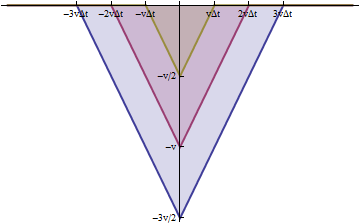
\includegraphics[width=0.5\textwidth]{images/png/for_deltac_force.png}
\end{center}

\textbf{3. Пусть:}
\[
	s(x, t) = \begin{cases}
	0, & x \notin [-l/2, l/2] \\
	S_0\eta(t - t_0)/l, & x \in [-l/2, l/2]
	\end{cases} =
	\frac{S_0}{l} [ \eta(x + l/2) - \eta(x - l/2)] \eta(t - t_0)
\]
что соответствует постоянной силе, действующей на участок струны.
\[
\begin{gathered}
	u(x, t) =
	-\frac{v}{2} \int\limits_{0}^{t} \! \int\limits_{-v\tau}^{v\tau} s(x - \xi, t - \tau) d\tau\, d\xi = 
	\\ =
	-\frac{v}{2} \int\limits_{0}^{t} \! \int\limits_{-v\tau}^{v\tau} \frac{S_0}{l} [ \eta(x + l/2 - \xi) - \eta(x - l/2 - \xi)]\eta(t - t_0 - \tau) d\tau\, d\xi = 
	\\ =
	-\frac{v}{2} \int\limits_{0}^{t - t_0} \! \int\limits_{-v\tau}^{v\tau} \frac{S_0}{l} [ \eta(x + l/2 - \xi) - \eta(x - l/2 - \xi)] d\tau\, d\xi = 
	-\frac{v}{2}\frac{S_0}{l} \int\limits_{S} d\tau\, d\xi
\end{gathered}
\]
Область интегрирования $S$ приведена на рисунке, и представляет собой пересечение полосы шириной $l$ и треугольника, ограниченного кривыми $y = v(t - t_0)$, $y = x$, $y = -x$.
\begin{center}
	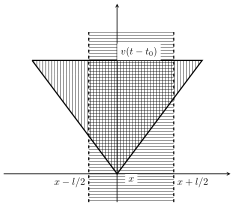
\includegraphics{images/png/for_example3.png}
	%\usetikzlibrary{patterns}
\begin{tikzpicture}

\draw[thick,-stealth]  (0,-1) -- (0,6);
\draw[thick,-stealth] (-4,0) -- (4,0);
\draw[very thick, pattern=vertical lines] (-3,4) -- (3, 4) -- (0,0) -- (-3, 4);
\draw[very thick, dashed] (2, -1) -- (2, 5);
\draw[very thick, dashed] (-1, -1) -- (-1, 5);
\path[pattern=horizontal lines] (2, -1) rectangle (-1, 5);

\node[below, fill = white] at (0.5,0) {$x$};
\node[above right, fill = white] at (0,4) {$v(t - t_0)$};
\node[below left] at (-1,0) {$x - l/2$};
\node[below right] at (2,0) {$x + l/2$};

\end{tikzpicture}
\end{center}
Решение можно представить с помощью функций, определяющих площадь пересечения треугольника с левой полуплоскостью, заданной прямой параллельной оси ординат:
\[
\begin{aligned}
& S_+(x, x_A, x_B, x_C, y_B) =  
\frac{1}{2} y_B \frac{(x - x_A)^2}{x_B - x_A} \eta(x - x_A) \eta(x_B - x)  + \\ & +
\frac{1}{2} y_B \left[(x_B - x_A) + \frac{2 x_C - x - x_B}{x_C - x_B} (x - x_B)\right] \eta(x - x_B) \eta(x_C - x) +
\frac{1}{2} y_B (x_C - x_A) \eta(x - x_C)
\end{aligned}
\]
\[
	\begin{aligned}
	u(x, t) & = -\frac{v}{2}\frac{S_0}{l} [S_+(x + l/2, -v(t - t_0), 0, v(t-t_0), v(t - t_0)) - S_+(x - l/2, -v(t - t_0), 0, v(t-t_0), v(t - t_0))]
	\end{aligned}
\]
К сожалению, выражение слишком громоздко, и его трудно проверить. На рисунке приведена форма струны в различные моменты времени:
\begin{center}
	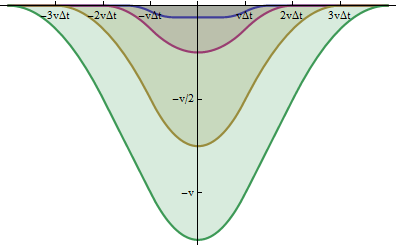
\includegraphics[width=0.5\textwidth]{images/png/for_const_force.png}
\end{center}
Примечательно, что сначала график пологий, но со временем приобретает более параболическую форму.

\textbf{4. Пусть:}

\[
s(x, t) = \delta(x - x_0) e^{i\omega t} \eta(t - t_0)
\]
что соответствует силе действующей в точке по синусоидальному закону.
\[
\begin{gathered}
u(x, t) =
-\frac{v}{4} \int\limits_{0}^{t} \! \int\limits_{-\infty}^{\infty} [ \sign (\xi + v \tau) - \sign (\xi - v\tau) ] s(x - \xi, t - \tau) d\tau d\xi =
\\ =
-\frac{v}{4} \int\limits_{0}^{t} \! \int\limits_{-\infty}^{\infty} [ \sign (\xi + v \tau) - \sign (\xi - v\tau) ] \delta(x - x_0 - \xi) e^{i\omega(t - \tau)} \eta(t - t_0 - \tau) d\tau d\xi =
\\ =
-\frac{v}{2} \eta(t - t_0) \int\limits_{0}^{t - t_0} \eta(v\tau - |x - x_0|) e^{i\omega(t - \tau)} d\tau =
-\frac{v}{2} \eta(t - t_0) \eta(t - t_0 - |x -x_0|/v) e^{i\omega t} \int\limits_{|x - x_0|/v}^{t - t_0} e^{-i\omega\tau} d\tau =
\\ =
\frac{v}{2i\omega} \eta(t - t_0) \eta(t - t_0 - |x -x_0|/v) e^{i\omega t} e^{-i\omega(t - t_0 - |x - x_0|/v)} =
\frac{v}{2i\omega} \eta(t - t_0) \eta(t - t_0 - |x -x_0|/v) \left(e^{i\omega t_0} - e^{i\omega(t - |x - x_0|/v)} \right)
\end{gathered}
\]
Проверяем:
\[
\begin{aligned}
& (\eta(t - t_0) \eta(t - t_0 - |x -x_0|/v) e^{i\omega|x - x_0|/v})'_x = 
\eta(t - t_0) (-\delta(t - t_0 - |x - x_0|/v) + i \omega )e^{i\omega|x - x_0|/v}\sign(x -x_0)/v
\end{aligned}
\]
\[
\begin{aligned}
& (\eta(t - t_0) \eta(t - t_0 - |x -x_0|/v) e^{i\omega|x - x_0|/v})''_{xx} = 
\eta(t - t_0) \delta'(t - t_0 - |x - x_0|/v) e^{i\omega|x - x_0|/v} \sign^2(x -x_0)/v^2 +
\\ & +
\eta(t - t_0) (-\delta(t - t_0 - |x - x_0|/v) + i \omega ) e^{i\omega|x - x_0|/v} i\omega \sign^2(x -x_0)/v^2 +
\\ & +
\eta(t - t_0) (-\delta(t - t_0 - |x - x_0|/v) + i \omega ) e^{i\omega|x - x_0|/v} 2\delta(x - x_0)/v
\end{aligned}
\]
\[
\begin{aligned}
& (\eta(t - t_0) \eta(t - t_0 - |x -x_0|/v) e^{i\omega|x - x_0|/v})'_{t} = 
\eta(t - t_0) \delta(t - t_0 - |x - x_0|/v) e^{i\omega|x - x_0|/v} +  
\\ & +
\eta(t - t_0 - |x - x_0|/v) \delta(t - t_0)e^{i\omega|x - x_0|/v} =
\eta(t - t_0) \delta(t - t_0 - |x - x_0|/v) e^{i\omega|x - x_0|/v} + \eta(- |x - x_0|/v)\delta(t - t_0)
\end{aligned}
\]
\[
\begin{aligned}
& (\eta(t - t_0) \eta(t - t_0 - |x -x_0|/v) e^{i\omega|x - x_0|/v})''_{tt} = 
\\ & = 
\eta(t - t_0) \delta'(t - t_0 - |x - x_0|/v) e^{i\omega|x - x_0|/v} + \delta(t - t_0) \eta(t - t_0 - |x -x_0|/v) e^{i\omega|x - x_0|/v} + 
\\ & +
\eta(- |x - x_0|/v)\delta'(t - t_0)
\end{aligned}
\]